\chapter{Background}
\section{Alzheimer's Disease}
Alzheimer's Disease (AD) is the most common cause of dementia, its incidence increases with age and it afflicts 6\% of the population aged over 65. \cite{Burns2009} It is characterised by cognitive dysfunction (loss of memory, language difficulties etc.), psychiatric symptoms (depression, hallucinations and delusions) known as non-cognitive symptoms. Severe cases may be unable to perform basic living tasks such as eating and dressing unaided. AD is a terminal disease, with death usually resulting from an associated condition such as complications of pressure ulcers or pneumonia that can manifest following the muscle atrophy that is typical in late-stage Alzheimer's patients.\cite{Burns2009}

Patients may become confused and aggressive. Interestingly these disruptive episodes have been shown to follow a temporal pattern, being more frequent in the late afternoon and early evening - a phenomenon known as `sundowning'. \cite{McCann2004} There is high comorbidity between AD and vascular disease to such an extent that the traditional distinction between AD and vascular disease as two separate diseases has been called into question.\cite{Stewart2002}

The shift from the normal cognitive decline expected with healthy ageing to preclinical dementia appears to be a gradual, continuous transition. The prodromal stage of AD is referred to as Mild Cognitive Impairment (MCI), it is characterised by memory impairments that would not be expected due to normal age-related related cognitive decline in the individual given their age and educational history (both are strong correlates for memory function). The status of MCI as a legitimate prodromal stage of AD rather than simply misdiagnosis of normal decline is supported by the fact that patients diagnosed with MCI are 15 times more likely to develop AD than those without a history of MCI.\cite{Burns2009}

Diagnosis is typically performed on the basis of cognitive and memory tests - the most common being the Mini Mental State Examination (MMSE) (see Figure \ref{fig:MMSEgraph}). Neuroimaging can aid diagnosis but no single modality has been proven as an accurate screening test. Neuroimaging used in cmbination with psychological testing outperforms either alone.\cite{Burns2009}


\begin{figure}[h!]
  \centering
    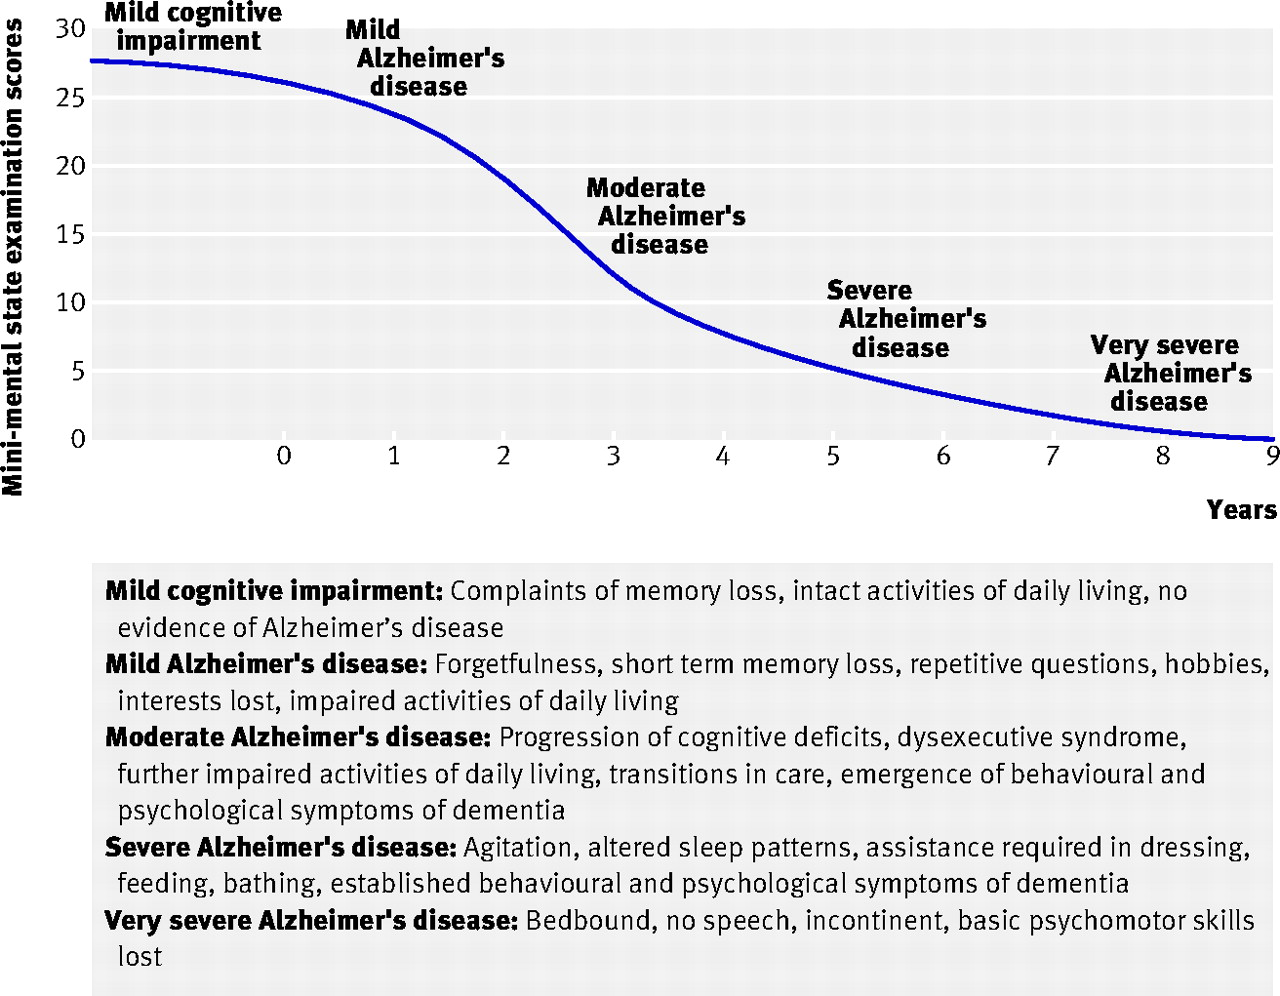
\includegraphics[width=\textwidth]{MMSEgraph.jpg}
    \caption{The progression of Alzheimer's Disease and the associated MMSE scores.\cite{Burns2009}}
    \label{fig:MMSEgraph}
\end{figure}

Although it is true that the there has been comparatively little progress in the search for an Alzheimer's cure compared to the improvement in diagnostic techniques the early diagnosis of MCI can help prevent misdiagnosis of AD and the selection of medical trial candidates. Furthermore, in the future it may allow preventative treatment to halt the progression or onset of the disease - given the modest success of late-stage intervention and the search for a cure there has been a great increase in interest concerning preventative treatment of Alzheimer's disease.\cite{Burns2009}






\section{Magnetoencephalography}

Magnetoencephalography (MEG) is a functional neuroimaging technique that measures the brain activity directly via measurement of the magnetic fields created by electrical currents at the synapses. This is a difficult task as the magnetic fields are extremely weak ($10-10^3$ fT) and thus requires the use of expensive and complicated neuromagnetometers which achieve their high sensitivity by the use of Superconducting Quantum Interference Devices (SQUIDs). Although it is worth mentioning that the first MEG recordings took place in the late 1960's before SQUIDs were available, instead using an induction coil magnetometer consisting of 2 million turns of copper wound about a ferrite core.\cite{Hari2012}

Furthermore the weakness of the magnetic fields relative to ambient magnetic noise ($10^8$ fT) requires shielding the laboratory to reduce noise. The magnetic field due to an electric current is described by Amp\`{e}re's Law and the direction can be easily determined by the right hand rule. As the magnetic field is orthogonal to the current, MEG is sensitive to the tangential component of the synaptic currents and therefore is most sensitive to pyramidal neurons near the cortical surface as pyramidal neurons have most of their currents tangential to the cortical surface and MEG is generally not sensitive to deep brain regions (although some studies have shown this may not always be the case\cite{Internationale2007}).

Despite these problems of MEG it has several advantages over other methods:

\begin{itemize}
\item It is non-invasive and has a high temporal resolution
\item Magnetic fields unlike electric fields in Electroencephalography (EEG) are not impeded by the skull, scalp etc.
\item Unlike EEG it does not require a reference signal allowing for easier source localisation\cite{Zani2002}
\item It is a direct measurement, unlike many methods such as fMRI and fNIRS which use cerebral blood flow as a proxy for neural activity

\end{itemize}

MEG recordings are often combined with anatomical MRI to enable accurate source localisation. The data processing requires the removal of artefacts which can be divided into three kinds: System related artefacts (Superconducting Quantum Interference Device (SQUID) jumps, nosiy/saturated channels etc.), external artefacts (due to power lines, mains AC etc.), physiological artefacts (due to eye movements, cardiac/muscle activity, head movement etc.). \cite{Gross2013} The visual inspection of raw data and power spectra is highly recommended although often automated/semi-automated approaches will have to be used due to the large volumes of data recorded. The way these challenges were handled in the present work will be discussed in the Methodology chapter.



\section{Previous work}


MEG has been used to investigate a wide range of brain disorders including Alzheimer's, Schizophrenia, Major Depressive Disorder and Autism. Techniques include synchrony and coherence studies (due to its high temporal resolution), Spectral ratios (the ratios of relative powers of the different frequency bands) and non-linear techniques such as complexity analysis.\cite{Williams2010}

As a result of these studies it was discovered that many brain disorders including Alzheimer's, depression, attention-deficit hyperactivity disorder and schizophrenia result in a change in the effect of ageing on brain activity as compared to healthy controls - this was described as a `rupture' in the normal evolution of the neural activity.\cite{Escudero2013}

Previous analysis on the dataset intended for use in this study found that brain oscillatory complexity (as quantified by the Lempel-Ziv Complexity algorithm) had a quadratic relationship with age.\cite{Fernandez2012} It was also discovered that spectral properties followed a similar quadratic relationship.\cite{Gomez2013}






